% !TEX program = pdflatex
% Manuscript section (SIAM-Review style, after Allard, Moore, Scarpino,
% Althouse & Hebert-Dufresne, SIAM Rev. 65 (2023) 471): concept-driven main
% text with the mathematics set off in numbered boxes.
%
% Compile:  pdflatex figure2_section  (needs figure2_lambda_c.pdf in the folder)
\documentclass[11pt]{article}
\usepackage[margin=1in]{geometry}
\usepackage{amsmath,amssymb,amsthm}
\usepackage{graphicx}
\usepackage[most]{tcolorbox}
\usepackage{bm}
\usepackage[hidelinks]{hyperref}
% Times-like fonts, close to the reference paper. Uncomment if `newtx` is
% installed; the section compiles fine with default fonts otherwise.
% \usepackage{newtxtext,newtxmath}

% ---- numbered "Box" environment, after the reference paper ---------------
\newcounter{sbox}
\newtcolorbox[use counter=sbox]{sbox}[1]{%
  breakable, colback=black!3, colframe=black!45, boxrule=0.5pt, arc=1.5pt,
  left=7pt, right=7pt, top=5pt, bottom=5pt, fonttitle=\bfseries,
  title={Box~\thesbox:\ #1}}

\newcommand{\avg}[1]{\langle #1 \rangle}
\newcommand{\kk}[1]{k^{(#1)}}
\newcommand{\one}{\bm{1}}
\newcommand{\Nmat}{\mathsf{N}}
\newcommand{\lc}{\lambda_c}
\newcommand{\Rinf}{R(\infty)}

\begin{document}

\section*{Locating the epidemic threshold from subcritical outbreaks}

Once the group closure has been reduced to its low-dimensional dynamical
system, the epidemic threshold $\lc$---the value of the single control
parameter $\lambda$ at which a vanishing seed can first ignite a macroscopic
outbreak---can be located in two logically independent ways. The first is
\emph{spectral}: one linearizes the branching process that carries the
infection from group to group and asks when its mean-offspring operator first
acquires a unit eigenvalue. The second, which we develop here and use as an
independent check, is \emph{thermodynamic} in spirit: one stays strictly below
threshold, measures how large the outbreak seeded by a small initial fraction
grows as $\lambda$ is raised, and reads $\lc$ off the divergence of that size.
Because the two routes share no intermediate quantity---one diagonalizes a
matrix built from the joint layer-degree distribution, the other integrates
the full nonlinear closure to its final state---their agreement is a
nontrivial test of both, and it is this comparison that Figure~\ref{fig:lc}
reports.

\paragraph{The model and its next-generation matrix.}
We spread a susceptible--infectious--recovered (SIR) process on a
\emph{multiplex hypergraph}: a node belongs to groups drawn from $M$ layers,
layer $a$ being a hypergraph of homogeneous group size $m_a$. A node's
participation is encoded by its layer-degree vector $\bm{k}=(\kk{1},\dots,\kk M)$,
with $\kk a$ the number of layer-$a$ groups it belongs to, distributed jointly
as $P(\bm{k})$; all inter-layer structure enters the theory only through the
moments $\avg{\kk a}$ and $\avg{\kk a \kk b}$. A group is \emph{active} once at
least $\theta_a$ of its members are infectious, whereupon it transmits to each
susceptible member at rate $\beta_a=\lambda w_a\mu$; infectious nodes recover
at rate $\mu$, so that after rescaling time the model carries the single scalar
control $\lambda$ (with fixed channel weights $w_a$). Fixing a cavity node and
tracking, for each of its groups, the joint count of susceptible, infectious
and recovered members yields a closed system of ordinary differential
equations whose dimension $\sum_a\binom{m_a+1}{2}+2$ is independent of the
population size $N$; its final state fixes the epidemic size through
$\Rinf=1-(1-\varepsilon)\,\Psi(\bm{\Phi}(\infty))$, where $\varepsilon$ is the
seeded fraction, $\Psi$ the node-side generating function, and $\Phi_a$ the
probability that a layer-$a$ group has not transmitted to the cavity node
(Box~\ref{box:model}).

\begin{sbox}{Group cascade and the next-generation matrix}\label{box:model}
The novelty of undirected groups is that a member infected inside a group
lengthens that group's active period and so raises the chance that its
remaining members are infected in turn---an \emph{intra-group cascade} absent
from the pairwise or directed picture. For a single seed in an isolated
$m$-group with threshold $\theta$, let $u(i,s)$ be the expected number of
\emph{further} infections started from $i$ infectious and $s$ susceptible
members. Writing $\alpha_i=\lambda s\,\mathbf 1[i\ge\theta]$ for the group's
total infection rate in units of the recovery rate,
\begin{equation}
u(i,s)=\frac{\alpha_i}{\alpha_i+i}\bigl[1+u(i+1,s-1)\bigr]
        +\frac{i}{\alpha_i+i}\,u(i-1,s),
\qquad u(0,s)=u(i,0)=0,
\label{eq:cascade}
\end{equation}
and the expected cascade size is the scalar $C(m,\lambda,\theta)=u(1,m-1)$. It
reduces to the pairwise transmissibility $C(2,\lambda,1)=\lambda/(1+\lambda)$,
exceeds the linear estimate $(m-1)\lambda/(1+\lambda)$ for $m\ge3$, and
vanishes for $\theta\ge2$ (a lone seed cannot activate the group).

The outbreak grows as a multi-type branching process whose types are the
layer through which a node was infected. A node reached through layer $a$
ignites, in each of its \emph{other} layer-$b$ groups, an expected
$C(m_b,\lambda_b,\theta_b)$ new infections, and it has on average
$\avg{\kk a\kk b}/\avg{\kk a}-\delta_{ab}$ such groups. The mean-offspring, or
next-generation, matrix is therefore
\begin{equation}
\Nmat_{ab}=C(m_b,\lambda_b,\theta_b)
      \left[\frac{\avg{\kk a\kk b}}{\avg{\kk a}}-\delta_{ab}\right],
\qquad \lambda_b=\lambda w_b ,
\label{eq:ngm}
\end{equation}
and the epidemic threshold is the value of $\lambda$ at which its spectral
radius reaches unity, $\rho(\Nmat)=1$. Setting all $m_a=2$ recovers the
next-generation matrix of multiplex network SIR, and $M=1,\ m=2$ recovers the
scalar configuration-model threshold $\avg{k}/(\avg{k^2}-\avg{k})$.
\end{sbox}

\paragraph{Reading the threshold off the subcritical outbreak size.}
Below threshold a small seed produces only a finite outbreak, but its expected
size grows without bound as $\lambda\to\lc^-$. Seeding a single random node,
the mean number of nodes it ever infects is, in the branching approximation,
\begin{equation}
\chi(\lambda)=\one^{\!\top}(\mathsf I-\Nmat)^{-1}\bm v_0
            =1+\one^{\!\top}(\mathsf I-\Nmat^{\!\top})^{-1}\bm g,
\qquad g_b=\avg{\kk b}\,C(m_b,\lambda_b,\theta_b),
\label{eq:chi}
\end{equation}
with $\bm v_0$ the seed's type distribution and $\bm g$ its first generation.
This mean size inherits its pole from $(\mathsf I-\Nmat)^{-1}$ and hence
diverges as $(1-\rho)^{-1}$ precisely where $\rho(\Nmat)=1$; note that it may
\emph{not} be replaced by the scalar $1/(1-\rho)$ except when $M=1$ or $\bm v_0$
is the Perron vector. The practical consequence is that its reciprocal is a
smooth function that crosses zero \emph{linearly} at the threshold, so that
$\lc$ is the zero-crossing of $\varepsilon/\Rinf$ (Box~\ref{box:extrap}). Since
$\Rinf$ is measured by integrating the full nonlinear closure---not by
diagonalizing $\Nmat$---this construction locates $\lc$ along a path that is
genuinely independent of the eigenvalue condition~\eqref{eq:ngm}.

\begin{sbox}{The subcritical extrapolation}\label{box:extrap}
For a set of subcritical values $\lambda<\lc$ we integrate the closure to its
final state and form the reciprocal outbreak size
\begin{equation}
y(\lambda)=\frac{\varepsilon}{\Rinf}=\frac{1}{\chi(\lambda)}
          \;\xrightarrow[\ \lambda\to\lc^-\ ]{}\; 0 ,
\qquad y(\lambda)\simeq c\,(\lc-\lambda)\ \ \text{near threshold,}
\label{eq:y}
\end{equation}
whose linear zero-crossing gives $\lc$. A finite seed rounds the transition
and leaves a nonzero $\Rinf$ exactly at $\lc$, biasing the crossing upward;
because $\Rinf/\varepsilon$ is linear in $\varepsilon$ for small seeds, this
bias is removed by a Richardson extrapolation $\varepsilon\to0$. As
$\varepsilon\to0$ the integrated final states converge onto the analytic
prediction~\eqref{eq:chi}---the relative gap falls from $3.7\times10^{-3}$ to
$1.1\times10^{-5}$ as $\varepsilon$ is halved from $2\times10^{-4}$ to
$10^{-5}$---confirming that the closure's subcritical size is exactly
$\one^{\!\top}(\mathsf I-\Nmat)^{-1}\bm v_0$ with its pole pinned to
$\rho(\Nmat)=1$.
\end{sbox}

\paragraph{Results.}
Figure~\ref{fig:lc} carries out this program for eight configurations whose
thresholds span $\lc\in[0.08,0.40]$ and include single-layer higher-order
hypergraphs, pairwise-degenerate networks, and two-layer multiplex hypergraphs.
Panel~(a) shows the reciprocal outbreak size $\varepsilon/\Rinf$ collapsing
linearly onto zero as $\lambda/\lc\to1$; the three examples reach the common
crossing (open circle) at the value predicted by $\rho(\Nmat)=1$. Panel~(b)
places the extrapolated threshold against the spectral one for all eight
configurations: they fall on the identity line, with a maximum relative
deviation of $6\times10^{-4}$. Panel~(c) expresses each deviation in units of
the regression standard error $\sigma$ of the extrapolated intercept; every
configuration lies within $1.5\sigma$ of $\rho(\Nmat)=1$. The small residual is
the expected finite-window curvature of~\eqref{eq:y}: the reciprocal size is
strictly linear only in the immediate neighborhood of $\lc$, so a fit over a
finite window carries a bias whose sign flips with the window's placement and
whose magnitude is comparable to $\sigma$, and therefore cannot be distinguished
from a genuine deviation.

Three further checks confirm that the agreement is not an artifact of the
closure. The within-group cascade $C(m,\lambda,\theta)$ of~\eqref{eq:cascade}
reproduces a direct single-group Gillespie simulation to within statistical
error ($\le\!1\sigma$ at $10^6$ realizations), including the analytic value
$\lambda/(1+\lambda)$ at $m=2$ and $C=0$ for $\theta\ge2$; the sum rule and the
all-susceptible identity of the closure hold at the $10^{-17}$ and $10^{-12}$
levels; and the disease-free Jacobian of the closure has its leading eigenvalue
cross zero exactly at $\rho(\Nmat)=1$ to machine precision. The subcritical
extrapolation thus provides a fully nonlinear, independent confirmation of the
spectral threshold, complementary to the Jacobian check, which probes only the
linearization.

\begin{figure}[t]
\centering
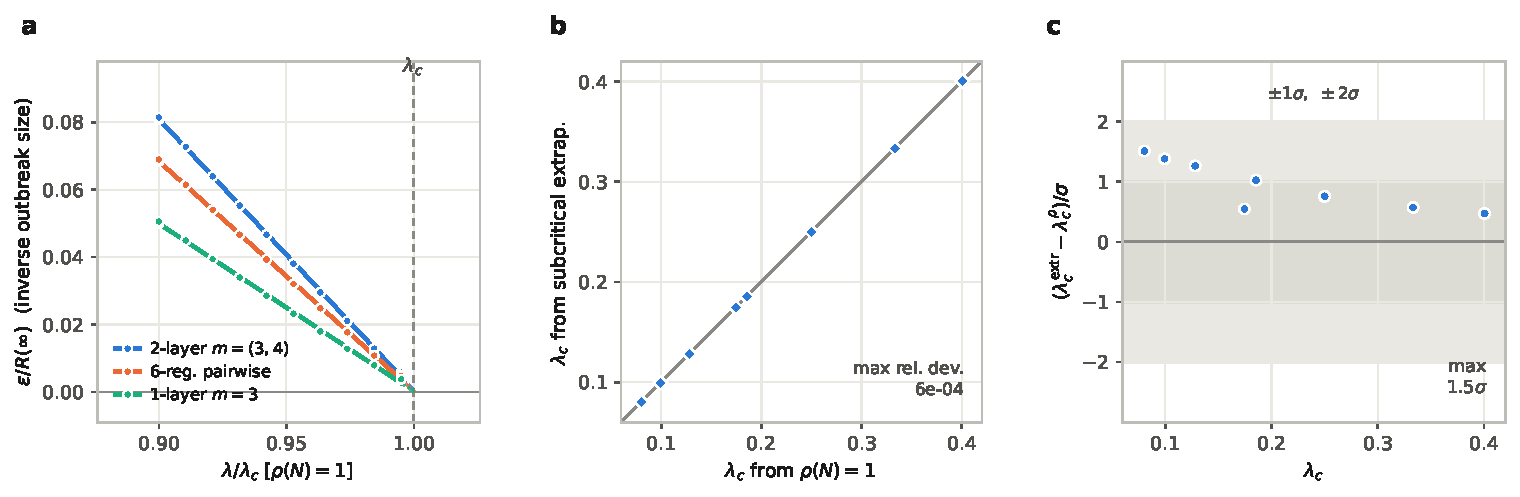
\includegraphics[width=\textwidth]{figure2_lambda_c.pdf}
\caption{\textbf{Locating the epidemic threshold $\lc$ by extrapolation from
subcritical final states, compared with the spectral condition
$\rho(\Nmat)=1$.} \textbf{(a)} The reciprocal mean outbreak size
$\varepsilon/\Rinf$ falls linearly to zero as the control parameter approaches
threshold, shown against the rescaled variable $\lambda/\lc$ for three
representative configurations (two-layer $m=(3,4)$, pairwise $6$-regular, and
single-layer $m=3$). Markers are the $\varepsilon\to0$ closure final states;
lines are linear fits over the near-threshold window
$[0.90,0.995]\,\lc$; the three fits meet the open circle at the point
$\rho(\Nmat)=1$ (dashed vertical marker). \textbf{(b)} Across eight
configurations the extrapolated threshold agrees with $\rho(\Nmat)=1$ along the
identity line, with maximum relative deviation $6\times10^{-4}$; error bars
(the regression standard error $\sigma$) are smaller than the markers.
\textbf{(c)} The deviation of each configuration in units of $\sigma$; all lie
within $1.5\sigma$ of the spectral prediction (shaded bands: $\pm1\sigma$,
$\pm2\sigma$). The uniformly positive, sub-$\sigma$ offset is the finite-window
curvature of the linear law~\eqref{eq:y}.}
\label{fig:lc}
\end{figure}

\end{document}
